\documentclass[11pt]{article}
\usepackage{fontspec}
\setmainfont{NotoSerif-Regular.ttf}[Path=C:/Windows/Fonts/,ItalicFont=NotoSerif-Italic.ttf,BoldFont=NotoSerif-Bold.ttf,BoldItalicFont=NotoSerif-BoldItalic.ttf]
\usepackage[a4paper,margin=22mm]{geometry}
\usepackage{amsmath,amssymb,graphicx,xcolor,hyperref,needspace,tikz}
\usepackage[normalem]{ulem}
\let\MathUnderline\underline
\renewcommand{\underline}[1]{\ifmmode\MathUnderline{#1}\else\uline{#1}\fi}
\hypersetup{unicode=true,colorlinks=true,linkcolor=blue,pdfauthor={}}
\setlength{\parindent}{0pt}
\setlength{\parskip}{.4em}
\setlength{\emergencystretch}{3em}
\raggedright
\newcommand{\SourcePage}[2]{\par\smallskip\phantomsection\label{#1:source-page}{\small\sffamily\color{blue!55!black}#1}\par\smallskip}
\newcommand{\EvidenceBlock}[4]{%
 \par\smallskip\noindent\begin{minipage}{\linewidth}
 \begin{minipage}[t]{.47\linewidth}\vspace{0pt}\centering
 \csname evidence-#1-#2\endcsname\par
 {\scriptsize\SourceCropCaption\ #1}\par
 \end{minipage}\hfill
 \begin{minipage}[t]{.49\linewidth}\vspace{0pt}\raggedright
 {\small\color{orange!65!black}\textbf{#4} #3}\par
 \end{minipage}
 \end{minipage}\par\smallskip}
\newcommand{\Unclear}[3]{\EvidenceBlock{#1}{#2}{#3}{\ReadingCaption}}
\newcommand{\Incomplete}[3]{\EvidenceBlock{#1}{#2}{#3}{\IncompleteCaption}}
\newcommand{\SourceFigure}[3]{\EvidenceBlock{#1}{#2}{#3}{\DiagramCaption}}
\expandafter\def\csname evidence-GELFAND-P000001-module-letter\endcsname{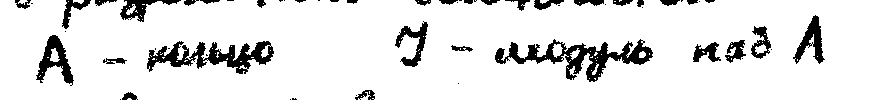
\includegraphics[width=\linewidth]{figures/gelfand-p000001-module-letter-original.png}}
\expandafter\def\csname evidence-GELFAND-P000001-diagram-blowup\endcsname{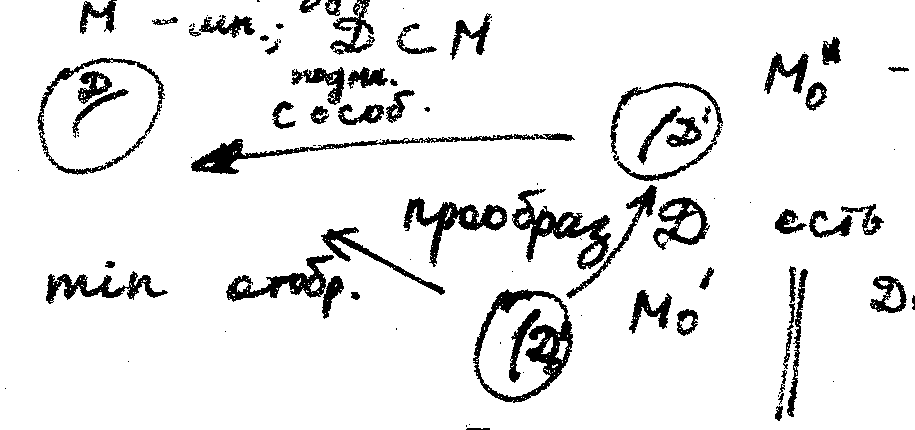
\includegraphics[width=\linewidth]{figures/gelfand-p000001-diagram-blowup-original.png}}
\expandafter\def\csname evidence-GELFAND-P000001-blowup-notation\endcsname{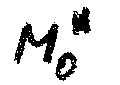
\includegraphics[width=.43\linewidth]{figures/gelfand-p000001-upper-blowup-label-original.png}\hfill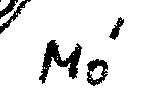
\includegraphics[width=.50\linewidth]{figures/gelfand-p000001-lower-blowup-label-original.png}}
\expandafter\def\csname evidence-GELFAND-P000001-origin-example\endcsname{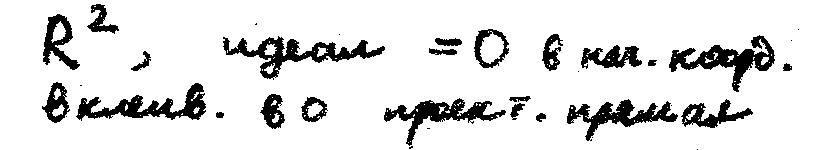
\includegraphics[width=\linewidth]{figures/gelfand-p000001-origin-example-original.png}}
\newcommand{\SourceCropCaption}{Оригинальные фрагменты:}\newcommand{\ReadingCaption}{Сомнительное чтение.}\newcommand{\IncompleteCaption}{Неразобранный фрагмент.}\newcommand{\DiagramCaption}{Рисунок и набранное описание.}
\hypersetup{pdftitle={Семинар И. М. Гельфанда — глава 1}}

\expandafter\def\csname evidence-GELFAND-P000002-ideal-selection\endcsname{
\includegraphics[width=\linewidth]{figures/gelfand-p000002-ideal-selection-part01-original-r1.png}}
\expandafter\def\csname evidence-GELFAND-P000002-open-set-notation\endcsname{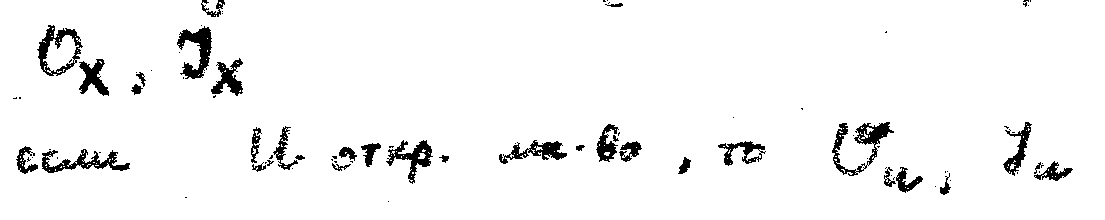
\includegraphics[width=\linewidth]{figures/gelfand-p000002-open-set-notation-part01-original-r2.png}}
\expandafter\def\csname evidence-GELFAND-P000002-fractions-sentence\endcsname{
\includegraphics[width=\linewidth]{figures/gelfand-p000002-fractions-sentence-part01-original-r1.png}\par\smallskip
\includegraphics[width=\linewidth]{figures/gelfand-p000002-fractions-sentence-part02-original-r1.png}\par\smallskip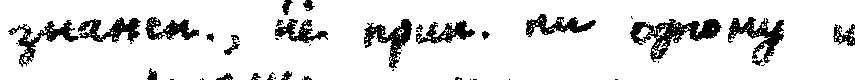
\includegraphics[width=\linewidth]{figures/gelfand-p000002-fractions-sentence-part03-original-r1.png}\par\smallskip
\includegraphics[width=\linewidth]{figures/gelfand-p000002-fractions-sentence-part04-original-r1.png}}
\expandafter\def\csname evidence-GELFAND-P000002-margin-grothendieck\endcsname{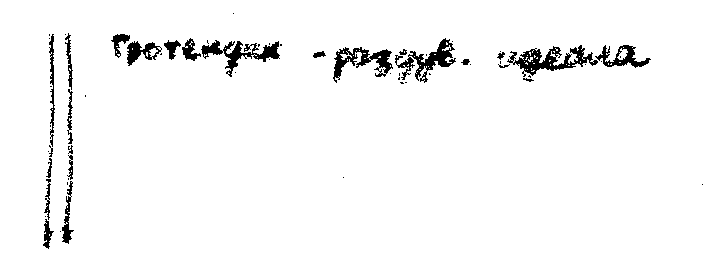
\includegraphics[width=\linewidth]{figures/gelfand-p000002-margin-grothendieck-part01-original-r1.png}}
\expandafter\def\csname evidence-GELFAND-P000002-quadratic-coefficients\endcsname{
\includegraphics[width=\linewidth]{figures/gelfand-p000002-quadratic-coefficients-part01-original-r1.png}}
\expandafter\def\csname evidence-GELFAND-P000002-last-sign\endcsname{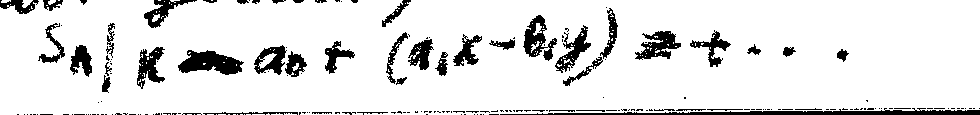
\includegraphics[width=\linewidth]{figures/gelfand-p000002-last-sign-part01-original-r1.png}}
\expandafter\def\csname evidence-GELFAND-P000003-directions\endcsname{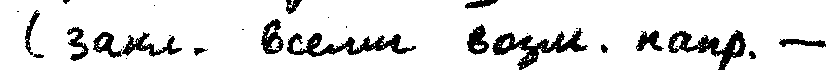
\includegraphics[width=\linewidth]{figures/gelfand-p000003-directions-part01-original-r1.png}\par\smallskip
\includegraphics[width=\linewidth]{figures/gelfand-p000003-directions-part02-original-r1.png}}
\expandafter\def\csname evidence-GELFAND-P000003-cross-cancellation\endcsname{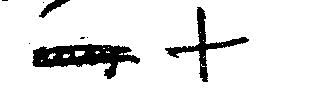
\includegraphics[width=\linewidth]{figures/gelfand-p000003-cross-cancellation-part01-original-r1.png}}
\expandafter\def\csname evidence-GELFAND-P000003-ising-cancellation\endcsname{
\includegraphics[width=\linewidth]{figures/gelfand-p000003-ising-cancellation-part01-original-r1.png}}
\expandafter\def\csname evidence-GELFAND-P000003-configuration-letter\endcsname{
\includegraphics[width=\linewidth]{figures/gelfand-p000003-configuration-letter-part01-original-r2.png}}
\expandafter\def\csname evidence-GELFAND-P000003-energy-cancellation\endcsname{
\includegraphics[width=\linewidth]{figures/gelfand-p000003-energy-cancellation-part01-original-r1.png}}
\expandafter\def\csname evidence-GELFAND-P000003-energy-case\endcsname{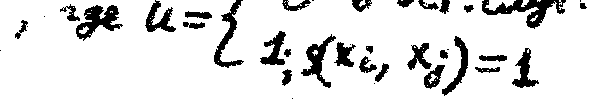
\includegraphics[width=\linewidth]{figures/gelfand-p000003-energy-case-part01-original-r2.png}\par\smallskip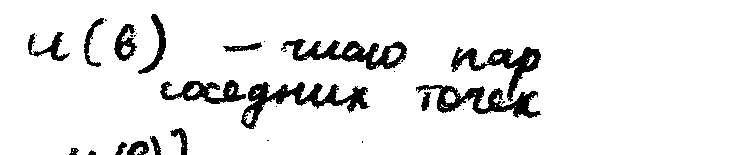
\includegraphics[width=\linewidth]{figures/gelfand-p000003-energy-case-part02-original-r3.png}}
\expandafter\def\csname evidence-GELFAND-P000003-partition-domain\endcsname{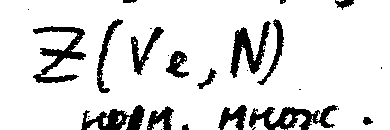
\includegraphics[width=\linewidth]{figures/gelfand-p000003-partition-domain-part01-original-r1.png}\par\smallskip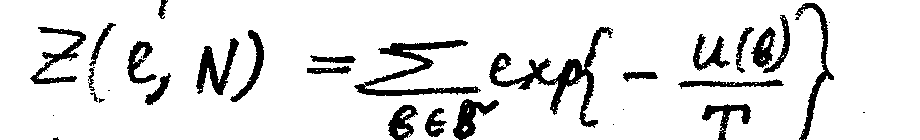
\includegraphics[width=\linewidth]{figures/gelfand-p000003-partition-domain-part02-original-r1.png}}
\expandafter\def\csname evidence-GELFAND-P000003-attraction-note\endcsname{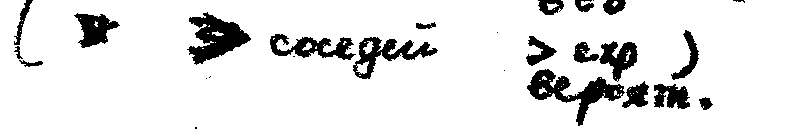
\includegraphics[width=\linewidth]{figures/gelfand-p000003-attraction-note-part01-original-r1.png}}
\expandafter\def\csname evidence-GELFAND-P000003-density-cancellation\endcsname{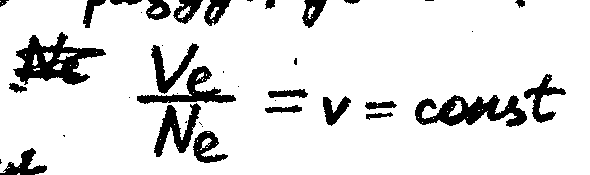
\includegraphics[width=\linewidth]{figures/gelfand-p000003-density-cancellation-part01-original-r1.png}}

\expandafter\def\csname evidence-GELFAND-P000004-pressure-letter\endcsname{
\includegraphics[width=\linewidth]{figures/gelfand-p000004-pressure-letter-part01-original-r1.png}}
\expandafter\def\csname evidence-GELFAND-P000004-diagram-phase-point\endcsname{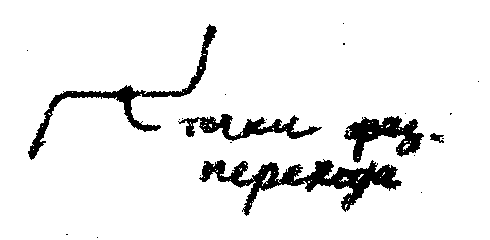
\includegraphics[width=\linewidth]{figures/gelfand-p000004-diagram-phase-point-part01-original-r2.png}}
\expandafter\def\csname evidence-GELFAND-P000004-diagram-cancelled-graph\endcsname{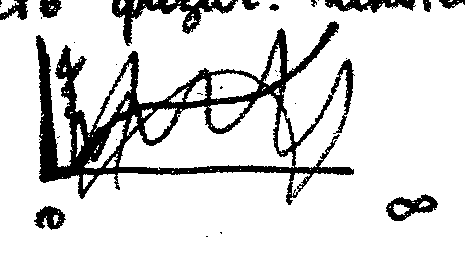
\includegraphics[width=\linewidth]{figures/gelfand-p000004-diagram-cancelled-graph-part01-original-r1.png}}
\expandafter\def\csname evidence-GELFAND-P000004-diagram-onsager\endcsname{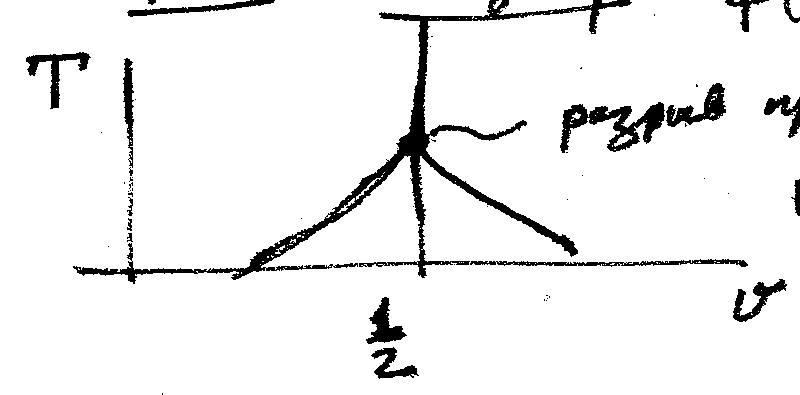
\includegraphics[width=\linewidth]{figures/gelfand-p000004-diagram-onsager-part01-original-r1.png}}
\expandafter\def\csname evidence-GELFAND-P000004-kac-helfand-note\endcsname{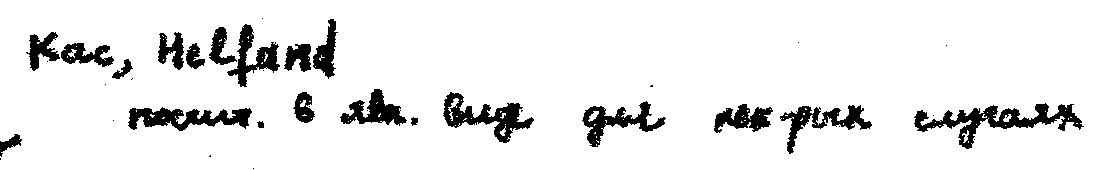
\includegraphics[width=\linewidth]{figures/gelfand-p000004-kac-helfand-note-part01-original-r1.png}}
\expandafter\def\csname evidence-GELFAND-P000004-diagram-subcube\endcsname{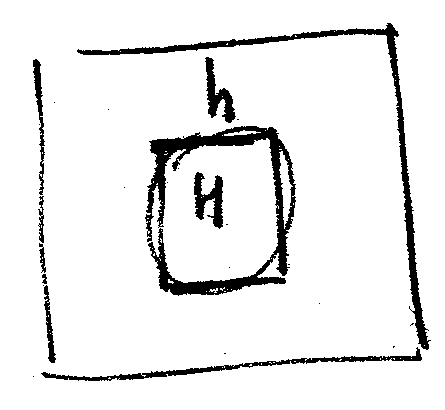
\includegraphics[width=\linewidth]{figures/gelfand-p000004-diagram-subcube-part01-original-r1.png}}
\expandafter\def\csname evidence-GELFAND-P000004-probability-bar\endcsname{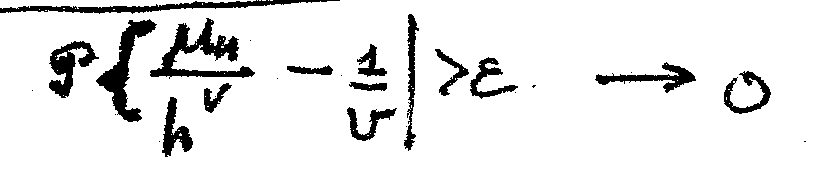
\includegraphics[width=\linewidth]{figures/gelfand-p000004-probability-bar-part01-original-r1.png}}
\expandafter\def\csname evidence-GELFAND-P000004-bottom-mark\endcsname{
\includegraphics[width=\linewidth]{figures/gelfand-p000004-bottom-mark-part01-original-r1.png}}
\expandafter\def\csname evidence-GELFAND-P000004-margin-left\endcsname{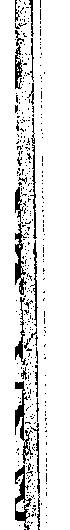
\includegraphics[height=60mm]{figures/gelfand-p000004-margin-left-part01-original-r1.png}\hspace{2mm}
\includegraphics[height=60mm]{figures/gelfand-p000004-margin-left-part02-original-r1.png}\hspace{2mm}
\includegraphics[height=60mm]{figures/gelfand-p000004-margin-left-part03-original-r1.png}\hspace{2mm}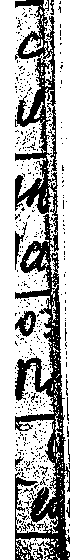
\includegraphics[height=60mm]{figures/gelfand-p000004-margin-left-part04-original-r1.png}}
\expandafter\def\csname evidence-GELFAND-P000005-exponential-rate\endcsname{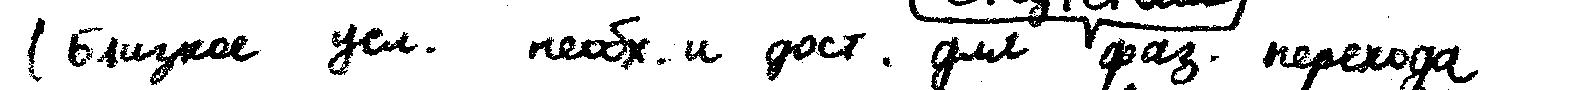
\includegraphics[width=\linewidth]{figures/gelfand-p000005-exponential-rate-part01-original-r1.png}\par\smallskip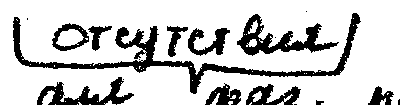
\includegraphics[width=\linewidth]{figures/gelfand-p000005-exponential-rate-part02-original-r1.png}\par\smallskip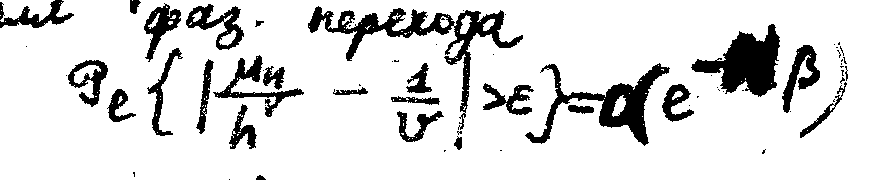
\includegraphics[width=\linewidth]{figures/gelfand-p000005-exponential-rate-part03-original-r2.png}}
\expandafter\def\csname evidence-GELFAND-P000005-complement-label\endcsname{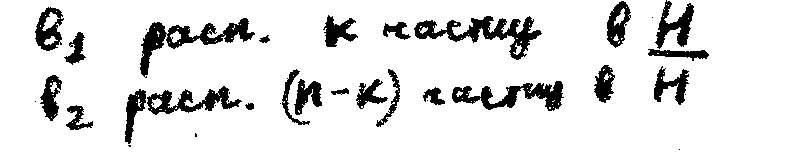
\includegraphics[width=\linewidth]{figures/gelfand-p000005-complement-label-part01-original-r1.png}}
\expandafter\def\csname evidence-GELFAND-P000005-boundary-exponent\endcsname{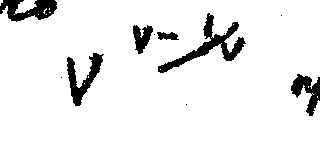
\includegraphics[width=\linewidth]{figures/gelfand-p000005-boundary-exponent-part01-original-r1.png}\par\smallskip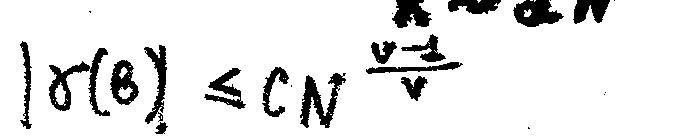
\includegraphics[width=\linewidth]{figures/gelfand-p000005-boundary-exponent-part02-original-r1.png}}
\expandafter\def\csname evidence-GELFAND-P000005-theta-factor\endcsname{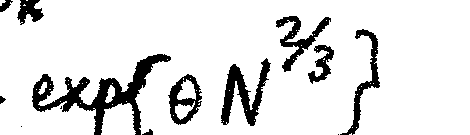
\includegraphics[width=\linewidth]{figures/gelfand-p000005-theta-factor-part01-original-r1.png}\par\smallskip
\includegraphics[width=\linewidth]{figures/gelfand-p000005-theta-factor-part02-original-r1.png}\par\smallskip
\includegraphics[width=\linewidth]{figures/gelfand-p000005-theta-factor-part03-original-r1.png}}
\expandafter\def\csname evidence-GELFAND-P000005-physical-meaning-heading\endcsname{
\includegraphics[width=\linewidth]{figures/gelfand-p000005-physical-meaning-heading-part01-original-r1.png}}
\expandafter\def\csname evidence-GELFAND-P000004-diagram-pressure-plateau\endcsname{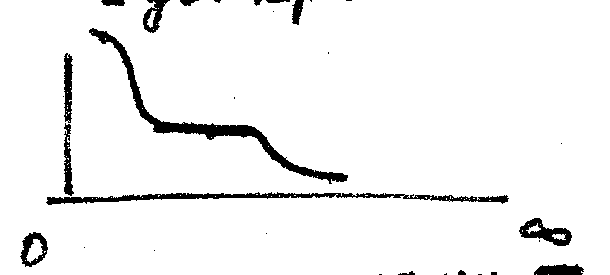
\includegraphics[width=\linewidth]{figures/gelfand-p000004-diagram-pressure-plateau-original-r1.png}}
\newcommand{\PhaseWords}{точки фаз.\\перехода}
\begin{document}
{\large\bfseries Семинар Гельфанда — глава 1}\par
{\small Начало читательского издания. Исходные страницы 1–5. Текст и формулы набраны; каждое сомнительное чтение сопровождается исходным фрагментом. Рабочий отрывок; полная глава готовится.}\par\medskip
\SourcePage{GELFAND-P000001}{unlabelled}
Понед. $21/\mathrm{IX}$.
Декартовы и булевы произв. групп.

«Хиронака: о разрешении особенностей».
\underline{Гельфанд}

$A$ — кольцо, $\mathcal{J}$ — модуль над $A$.
\Unclear{GELFAND-P000001}{module-letter}{Буква модуля и идеала передана как $\mathcal{J}$; возможны $\mathcal{I}$ или $J$.}

Раздутие — ?
$M$ — мн.; $D\subset M$.
[Под $D$:] подмн. с особ.

$M_0^H$ — раздутие. Blowing-up.
Прообраз $D$ есть $D'$ мн. разм. $n-1$.
$D_0$ — $(n-1)$-мерное.
\SourceFigure{GELFAND-P000001}{diagram-blowup}{Три обведённых рисунка: слева область с $D$, справа сверху область с $D'$ и подписью $M_0^H$, справа снизу область и подпись $M'_0$. Верхняя стрелка направлена влево; нижняя наклонная стрелка также влево, с подписью «непр. отобр.». Точные внутренние кривые, подписи и соединение нижней области с верхней требуют сравнения со сканом.}
\Unclear{GELFAND-P000001}{blowup-notation}{Верхний индекс у $M_0$ похож на $H$; подпись нижней области похожа на $M'_0$.}

Конструкция — Гротендик.
$A$ — кольцо, $\mathcal{J}$ — модуль.
\underline{Прим.} $A$ — кольцо ф-й;
$\mathcal{J}$ — идеал ф-й, обр. в $0$ на $D$.

Получится пучок колец и пучок модулей.
$A$ — кольцо, $\mathcal{J}$ — идеал.
Построим $X$, $O_X$ — пучок колец,
$\mathcal{J}_X$ — пучок идеалов, чтобы
\begin{gather*}
 (A,\mathcal{J})\ \longleftarrow\ (X,O_X,\mathcal{J}_X).
\end{gather*}
[Под стрелкой:] лин. отобр.

$(A,\mathcal{J})$ — пучок, порожд. $1$-м ид.

$\mathcal{J}_X$ обратим, т. е. идеал кольца:
$\exists f\in\mathcal{J}_X$ такого, что $O_Xf=\mathcal{J}_X$.
[Над формулой, стрелка к $\exists$:] образ.

(Идеал — главный, если $\mathcal{J}$ — идеал.)
Тогда многообр. нулей — $1$ ур-е.

$A$ — кольцо, $\mathcal{J}$ — идеал.
\underline{Тип. пример:} $R^2$, идеал $=0$ в нач. коорд.
\Unclear{GELFAND-P000001}{origin-example}{Следующая строка: «Вклеив. в $0$ проект. прямой»; начало может читаться «Оклеив.».}

$A$, $\mathcal{J}$ — мод.
\begin{gather*}
 \mathcal{J}\otimes_A\mathcal{J},\qquad
 \mathcal{J}\otimes_A\mathcal{J}\otimes_A\mathcal{J},\ldots
\end{gather*}
[Над группами тензорных произведений:] симм.; симм.

Рассм. форм. суммы
\begin{gather*}
 \sum_{k=0}^{N}a_kz^k.
\end{gather*}
Склад. и умн.
$x\otimes y=y\otimes x$.
\begin{gather*}
 a_0\in A,\qquad a_1\in\mathcal{J},\qquad
 a_2\in\mathcal{J}\otimes_A\mathcal{J}\quad\text{—}
\end{gather*}

\SourcePage{GELFAND-P000002}{unlabelled}
Кольцо таких сумм $S_A(\mathcal{J})$.
Рассм. однор. идеалы
[над строкой вставлено:] (градуир.).
(Вместе с многочленом сод. все его однородные.)

Рассм. все простые однор. идеалы в $S_A(\mathcal{J})$.
Выбр. идеалы, к-рые сод. все мн., нач. с $1$-й степени.
\Unclear{GELFAND-P000002}{ideal-selection}{Конец строки после «сод. все» лучше читается как «мн., нач. с $1$-й степени»; средние штрихи сокращения «нач.» остаются не вполне различимыми.}

Совок. идеалов $X$. (Топология Зарисского.)
$O_X$, $\mathcal{J}_X$.
Если $U$ откр. мн-во, то $O_U$, $\mathcal{J}_U$.
\Unclear{GELFAND-P000002}{open-set-notation}{После «то» первая буква совпадает по форме с $O_X$ выше, вторая — с буквой идеала: $O_U$, $\mathcal{J}_U$; последняя может быть $\mathcal{I}_U$.}

$S_A(\mathcal{J})$ — всё кольцо.
Кольцо отношений, числ., знамен., не прин. ни одному из идеалов.
Локализ. кольцо на это мн-во.
Отнош. $1$-й степени $\mathcal{J}_U$.
\Unclear{GELFAND-P000002}{fractions-sentence}{В строке об отношениях не вполне ясны сокращения «числ.-знамен.» и то, относится ли «не прин.» только к знаменателю. Слова не дополнены по смыслу.}
[Справа, две стрелки вниз:] Гротендик — раздуть идеально.
\Unclear{GELFAND-P000002}{margin-grothendieck}{Правая помета читается как «Гротендик — раздуть идеально»; последнее слово возможно «идеально» или «идеалы».}

$A$ — кольцо многочл. $2$-х пер.
$\mathcal{J}$ — идеал из мн. $P(0,0)=0$.
\begin{gather*}
 A=\{P(x,y)\},\qquad
 \mathcal{J}=P(x,y)=a_1x+b_1y+\cdots .
\end{gather*}
\begin{gather*}
 \mathcal{J}\otimes_A\mathcal{J}\ \longleftrightarrow
 \{a_2x^2+2b_2xy+cy^2+\cdots\}.
\end{gather*}
\Unclear{GELFAND-P000002}{quadratic-coefficients}{Коэффициенты в квадратном многочлене читаются $a_2$, $2b_2$, $c$; индекс у $c$ и вид толстой двусторонней стрелки не уверены.}

Из-за переброски получ. то же, что квадрат идеала.
Тогда — идеал из мн., равных $0$ в этой точке.
Во что она раздуется? ?

\begin{gather*}
 \sum P_k(x,y)z^k,\qquad P_k(x,y)=ax^k+\cdots .
\end{gather*}
[Справа:] Градуир. $\Sigma$ тенз. произвед.
\begin{gather*}
 A=\{P_0(x,y)\}\longrightarrow S_A(\mathcal{J}),\qquad
 P_0(x,y)\sim P_0(x,y).
\end{gather*}
Набор простых идеалов, получ. из ид. $P(0,0)=0$.
\begin{gather*}
 S_A\sim\sum P_kz^k,\qquad P_k\in\mathcal{J}^k,\qquad
 K\sim\sum P_kz^k.
\end{gather*}
Дост. найти max ид. факторкольца —
(чтобы найти ид., сод. данный).
\begin{gather*}
 S_A/K\ \longleftrightarrow\ a_0+(a_1x-b_1y)z+\cdots .
\end{gather*}
\Unclear{GELFAND-P000002}{last-sign}{В последней формуле перед $b_1y$ виден минус, хотя на следующем скане стоит плюс. Сохранён видимый минус; направление толстой стрелки также не вполне ясно.}

\SourcePage{GELFAND-P000003}{2}
Все однор. max ид. в нём и будут точками расширения.
Своб. члена нет (тогда и $1$).
\begin{gather*}
 (a_1x+b_1y)z.
\end{gather*}
Только $1$ лин. комб. $x$ и $y$.
($2$ нет, т. к. тогда все.)

Идеалы опр. напр. на плоскости
(замк. всеми возм. напр. — $\sigma$-процесс).
\Unclear{GELFAND-P000003}{directions}{Сокращения в скобках читаются «замк. всеми возм. напр.»; первое слово и значение знака $\sigma$ не утверждаются.}
\Needspace{48mm}\underline{Задача.} В пр-ве
[зачёркнуто:] \Unclear{GELFAND-P000003}{cross-cancellation}{Зачёркнутое слово перед рисунком не читается.}
\par\smallskip\noindent\begin{minipage}{\linewidth}\begin{minipage}[t]{.47\linewidth}\centering\vspace{0pt}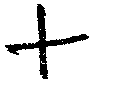
\includegraphics[width=30mm]{figures/gelfand-p000003-cross-diagram-original-r1.png}\par{\scriptsize Исходный рисунок}\end{minipage}\hfill\begin{minipage}[t]{.49\linewidth}\centering\vspace{0pt}\begin{tikzpicture}[scale=0.5]
 \draw (-0.8,0)--(0.8,0);
 \draw (0,-0.7)--(0,0.8);
\end{tikzpicture}\par{\scriptsize Наборное воспроизведение}\end{minipage}\end{minipage}\par\smallskip
Что получ. при заклеивании?
\begin{gather*}
 z=0,\qquad xy=0,\qquad \mathcal{J}=(z,xy).
\end{gather*}
[Под системой проведена черта.]

\underline{Добрушин.}
[Зачёркнуто перед «Найти»:] \Unclear{GELFAND-P000003}{ising-cancellation}{Зачёркнутое начало строки не читается уверенно.}
Найти пример газа, в к-ром сущ. фаз. переходы.
Куб целочисл. решётки.
$\ell$ — длина. $V_\ell=\ell^\nu$.
$N$ точ. $N<V_\ell$.
Могут заним. полож. на решётке
$\theta=(x_1,\ldots,x_N)$.
\Unclear{GELFAND-P000003}{configuration-letter}{Знак конфигурации передан как $\theta$; рукописный знак также похож на $b$ или кириллическое «в».}

Модель Изинга.
[Перед формулой густой зачёркнутый знак:]
\Unclear{GELFAND-P000003}{energy-cancellation}{Отдельный зачёркнутый знак перед $U(\theta)$ не читается.}
\begin{gather*}
 U(\theta)=-\frac12\sum_{i\ne j}u(x_i,x_j),\qquad
 u=\begin{cases}
 0&\text{в ост. случ.},\\
 1;&\rho(x_i,x_j)=1.
 \end{cases}
\end{gather*}
$u(\theta)$ — число пар соседних точек.
\Unclear{GELFAND-P000003}{energy-case}{В условии второй ветви виден знак, похожий на $\rho$; точка с запятой после $1$ сохранена. В подписи ниже первая буква похожа на малое $u$, а не $U$.}

Осн. аксиом — распр. Гиббса.
\begin{gather*}
 \mathsf{P}(B)=
 \frac{\displaystyle\sum_{\theta\in B}\exp\{-U(\theta)/T\}}
 {Z(V_\ell,N)},\qquad T>0\text{ — темпер.}
\end{gather*}
[Под знаменателем:] норм. множ.
\begin{gather*}
 Z(\ell,N)=\sum_{\theta\in\mathcal{B}}\exp\{-U(\theta)/T\}.
\end{gather*}
\Unclear{GELFAND-P000003}{partition-domain}{В знаменателе первой формулы написано $Z(V_\ell,N)$, следующая строка — $Z(\ell,N)$; знак множества под суммой похож на $\mathcal{B}$. Не исправлено по согласованности.}

Молекулы притяг.
([Два закрашенных знака со стрелками:] соседи $>$ их вероятн.)
\Unclear{GELFAND-P000003}{attraction-note}{В скобках после «Молекулы притяг.» закрашенные знаки и стрелки; чтение «соседи $>$ их вероятн.» не уверено.}
$B\subset\mathcal{B}$ — совок. распол.
\begin{gather*}
 p(\theta)=\frac{\exp\{-U(\theta)/T\}}{Z(\ell,N)}.
\end{gather*}
Пред. перех. $\ell\to\infty$, куб раздув. до $\infty$.
$N_\ell$ зав. от $\ell$.
[Зачёркнутый знак перед дробью:]
\Unclear{GELFAND-P000003}{density-cancellation}{Зачёркнутый знак перед $V_\ell/N_\ell$ не читается.}
\begin{gather*}
 \frac{V_\ell}{N_\ell}=v=\mathrm{const}.
\end{gather*}
Реш. увеличивается.
Можно показ., что
\begin{gather*}
 \frac1{N_\ell}\log Z(\ell,N_\ell)\longrightarrow f(v,T).
\end{gather*}

\SourcePage{GELFAND-P000004}{unlabelled}
\begin{gather*}
 p(v,T)=T\frac{\partial f}{\partial v}\qquad\text{по опред.}
\end{gather*}
\Unclear{GELFAND-P000004}{pressure-letter}{В первом аргументе $p$ густой знак похож на $v$; перед производной минус не виден и не добавлен.}

Фаз. переход.
По поводу $f$ — это монот., выпуклая ф-я по $v$.
Поэтому $p>0$ и $p$ монот. ф-я $v$.
Фаз. переход: $p(v,T)$ им. плоский участок.
\SourceFigure{GELFAND-P000004}{diagram-phase-point}{В правом верхнем поле ломаная S-подобная кривая с почти горизонтальным средним отрезком и стрелкой к нему; подпись «точки фаз. перехода». Точные оси и точки на исходном рисунке не обозначены уверенно.\par\smallskip\centering\resizebox{.93\linewidth}{!}{\begin{tikzpicture}[x=1cm,y=1cm]
\draw[thick] (0,0)..controls(.25,.2)and(.25,.85)..(.55,.9)--(2.25,.9)..controls(2.7,.9)and(2.55,1.4)..(2.8,1.8);
\fill(1.35,.9)circle(1.8pt);
\draw[thick](1.35,.87)..controls(1.35,.47)and(1.5,.45)..(1.9,.45);
\node[anchor=west,align=left,font=\small]at(2.15,.25){\PhaseWords};
\end{tikzpicture}}\par{\scriptsize Наборная схема; ограничения указаны в примечании.}\par}
Есть физич. гипотеза — $1$ уч. перех.

\SourceFigure{GELFAND-P000004}{diagram-cancelled-graph}{Слева график с вертикальной и горизонтальной осями, $0$ и $\infty$ у горизонтальной оси. Несколько кривых и прямых густо перечёркнуты; точная зачёркнутая кривая и вертикальная подпись требуют проверки.\par\smallskip\centering\resizebox{.93\linewidth}{!}{\begin{tikzpicture}[x=1cm,y=1cm]
\draw[thick](0,1.75)--(0,0)--(3.6,0);
\node[below]at(0,-.05){$0$};\node[below]at(3.6,-.05){$\infty$};
\end{tikzpicture}}\par{\scriptsize Частичное воспроизведение: только уверенные оси; зачёркнутые кривые не восстановлены.}\par}
\SourceFigure{GELFAND-P000004}{diagram-pressure-plateau}{Соседний рисунок справа: чистая убывающая кривая с плоским участком. Это отдельный график, а не восстановление зачёркнутого рисунка слева.\par\smallskip\centering\resizebox{.9\linewidth}{!}{\begin{tikzpicture}[scale=0.7]
 \draw (0,0)--(4.6,0);
 \draw (0,0)--(0,2.3);
 \draw (0.2,2.5).. controls (0.9,2.4) and (0.5,1.25)..(1.2,1.15)
 --(2.4,1.15).. controls (2.9,1.05) and (2.7,0.45)..(4,0.35);
 \node at (-0.1,-0.4) {$0$};
 \node at (4.6,-0.4) {$\infty$};
\end{tikzpicture}}\par{\scriptsize Прежнее наборное воспроизведение.}}
Плоский отр. есть при дост. малых $T$ ($<T_{\text{крит}}$).

Допускает явное реш. при $n=1$.
Считается $Z$ и $f(v,T)$.
Фаз. переходов нет, что счит. физич. естественным.

\underline{$n=2$.} \underline{Онзагер.}
$f(v,T)$ выч. для частных $v$ и $T$.
Разрыв производной соотв. фаз. переходам.
\SourceFigure{GELFAND-P000004}{diagram-onsager}{График с осью $T$ вверх, осью $v$ вправо, подписью $1/2$ под вертикалью через вершину. Кривая поднимается слева к вершине, убывает вправо; вертикальная линия проходит через вершину, справа от неё небольшой волнистый отрезок. Точная геометрия и значение волнистой ветви не установлены.\par\smallskip\centering\resizebox{.93\linewidth}{!}{\begin{tikzpicture}[x=1cm,y=1cm]
\draw(0,0)--(4.6,0);\draw(0,0)--(0,2.3);
\node[left]at(0,2.3){$T$};\node[below]at(4.6,0){$v$};
\draw(2.2,-.05)--(2.2,2.65);\node[below]at(2.2,-.12){$1/2$};
\draw[thick](.7,-.02)..controls(1.25,.35)and(1.85,.95)..(2.2,1.35)..controls(2.4,1.1)and(3.05,.55)..(3.45,.18);
\draw(1.05,.18)..controls(1.5,.54)and(1.9,1)..(2.17,1.35);
\fill(2.2,1.35)circle(1.5pt);
\draw[thick](2.32,1.4)..controls(2.5,1.62)and(2.63,1.33)..(2.78,1.42)..controls(2.86,1.47)and(2.98,1.56)..(3.03,1.61);
\end{tikzpicture}}\par{\scriptsize Наборная схема; ограничения указаны в примечании.}\par}

Kac, Helfand.
Точн. в яв. виду для нек-рых случаях.
\Unclear{GELFAND-P000004}{kac-helfand-note}{После повторного увеличения строка читается «точн. в яв. виду для нек-рых случаях»; возможны окончания «виде» и «случаев». Неграмматичное чтение не заменено автоматически.}

\SourceFigure{GELFAND-P000004}{diagram-subcube}{Большой квадрат и меньшая обведённая область внутри; в центре $H$, над малой областью $h$. Малый контур отчасти квадратный, отчасти округлый; точные границы не восстановлены.\par\smallskip\centering\resizebox{.93\linewidth}{!}{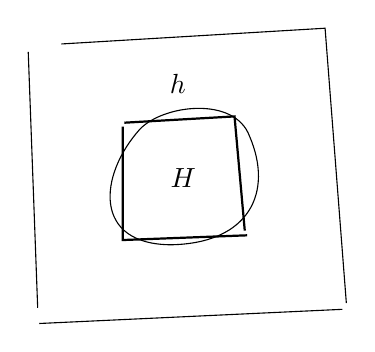
\begin{tikzpicture}[x=1cm,y=1cm]
\draw(.3,3.45)--(3.65,3.65)--(3.92,.16);\draw(3.87,.08)--(.02,-.1);\draw(0,.1)--(-.12,3.35);
\draw[thick](1.1,2.45)--(2.5,2.53)--(2.63,1.08);\draw[thick](2.66,1.02)--(1.08,.96)--(1.08,2.4);
\draw(1.3,2.37)..controls(1.6,2.68)and(2.5,2.79)..(2.69,2.28)..controls(3,1.56)and(2.68,.92)..(1.7,.9)..controls(.7,.9)and(.77,1.78)..(1.3,2.37);
\node at(1.85,1.75){$H$};\node at(1.78,2.94){$h$};
\end{tikzpicture}}\par{\scriptsize Наборная схема; ограничения указаны в примечании.}\par}
\begin{gather*}
 \frac{\mu_H}{h^\nu}.
\end{gather*}
$\mu_H$ — число частиц в $H$ — подкуб.
$\nu$ — размерность.
\begin{gather*}
 \frac{\mu_H}{h^\nu}=\frac1v\qquad\text{как и во всём пр-ве.}
\end{gather*}
\underline{Зак. больших чисел.}
\begin{gather*}
 \mathsf{P}\left\{\frac{\mu_H}{h^\nu}-\frac1v\,\middle|\,>\varepsilon\right\}
 \longrightarrow0.
\end{gather*}
\Unclear{GELFAND-P000004}{probability-bar}{В вероятностной формуле правая вертикальная черта перед $>\varepsilon$ видна, левая черта перед дробью не прочитана уверенно. Формула не дополнена молча парной чертой.}
\begin{gather*}
 \ell\to\infty,\qquad H\to\infty,\qquad
 d<\frac h\ell<1-d,\qquad d>0.
\end{gather*}
\Unclear{GELFAND-P000004}{bottom-mark}{У нижнего правого края небольшой знак похож на «2» или оборванную букву; как номер страницы не принят.}
\Incomplete{GELFAND-P000004}{margin-left}{Вдоль самого левого края видна узкая полоса соседнего рукописного текста, обрезанная до отдельных окончаний и штрихов; связный текст не читается.}



\SourcePage{GELFAND-P000005}{3}
Если это \underline{не} вып., то имеет место фазовый переход.
\Unclear{GELFAND-P000005}{physical-meaning-heading}{Нагл. [кандидат сокращения; средние штрихи не вполне различимы]} смысл. Сосущ. $2$ фазы, част. расп. неравномерно —
— жидкость и газ.
[Над строкой:] (зак. больш. чисел).
[Вставка над «фаз. перехода», со скобкой:] отсутствия.
(Близкое усл. необх. и дост. для фаз. перехода
\begin{gather*}
 \mathsf{P}_\ell\left\{\left|\frac{\mu_H}{h^\nu}-\frac1v\right|>\varepsilon\right\}
 =O(e^{-N\beta}).
\end{gather*}
\Unclear{GELFAND-P000005}{exponential-rate}{Показатель у $e$ содержит густо записанный знак перед $\beta$; кандидат $-N\beta$, но $N$ закрыт наложенными штрихами. Скобка, открытая перед «Близкое», на скане явно не закрыта.}
[Справа:] $N$ — число частиц.

Подсчит. вер., что
\begin{gather*}
 \mathsf{P}\{\mu_H=k\}=Z^{-1}
 \sum_{\theta\in\mathcal{B}_k}\exp\{-U(\theta)/T\}.
\end{gather*}
По распол., в к-рых в $H$ сидят $k$ частиц.
$\theta$ — распол. $N$ частиц.
$\theta\in\mathcal{B}_k$.
Тогда $\theta=(\theta_1,\theta_2)$.
$\theta_1$ расп. $k$ частиц в $H$.
$\theta_2$ расп. $(N-k)$ частиц в $\overline H$.
\Unclear{GELFAND-P000005}{complement-label}{У $H$ в строке про $\theta_2$ верхняя черта не вполне отчётлива; кандидат $\overline H$.}
\begin{gather*}
 U(\theta)=U(\theta_1)+U(\theta_2)+\gamma(\theta).
\end{gather*}
$U(\theta_1)$ — взаимод. внутри.
$U(\theta_2)$ — соседи вне.
$\gamma(\theta)$ — взаимод. через пов.
$\gamma(\theta)$ можно асимптотически пренебречь.
(Через гран. — пор. числа гран. точек)
$V^{\nu-1/\nu}$ при $N\to\infty$.
$k\sim dN$.
\Unclear{GELFAND-P000005}{boundary-exponent}{Степень у $V$ выглядит как $\nu-1/\nu$, без уверенно различимого общего числителя. Не заменена автоматически на $(\nu-1)/\nu$.}
\begin{gather*}
 |\gamma(\theta)|\le CN^{\frac{\nu-1}{\nu}}.
\end{gather*}
\begin{align*}
 \sum\exp\{-U(\theta)/T\}
 &=\sum_{\theta\in\mathcal{B}_k}\exp\{-U(\theta_1)/T\}
 \exp\{-U(\theta_2)/T\}\\
 &\qquad\times
 \exp\{\theta N^{2/3}\}
 =
\end{align*}
\Unclear{GELFAND-P000005}{theta-factor}{Буква перед $N^{2/3}$ похожа на $\theta$ или $\Theta$; на скане та же буква ниже пояснена «огранич. параметр». Она может отличаться от знака конфигурации.}
$\theta$ — огранич. параметр.
\begin{gather*}
 =\exp\{\theta N^{2/3}\}
 \sum_{\theta_1}\exp\{-U(\theta_1)/T\}
 \sum_{\theta_2}\exp\{-U(\theta_2)/T\}.
\end{gather*}
[Под первой суммой:] распол.


\clearpage\section*{Полные примечания к чтениям}
\subsection*{GELFAND-0001-U001}
\EvidenceBlock{GELFAND-P000001}{module-letter}{После A — кольцо стоит рукописная буква с развилкой сверху и нижним крюком; она повторяется у модуля и идеала.}{Наблюдение.}
\par\smallskip\noindent\textbf{Варианты: } \(\mathcal{J}\); \(\mathcal{I}\); J\par
\par\smallskip\noindent\textbf{Историческая помета: } В тексте использован каллиграфический J как графический кандидат; обозначение не определено по математическому смыслу.\par
\par\smallskip\noindent\textbf{Повторное сравнение: } В трёх отдельных вхождениях при 5×/10× видны развилка сверху и нижний крюк. Это подтверждает единое графическое обозначение,но не устанавливает однозначно условное различие I/J.\par
\subsection*{GELFAND-0001-U002}
\EvidenceBlock{GELFAND-P000001}{diagram-blowup}{В верхней половине три округлых контура с внутренними кривыми, две стрелки влево; над ними и рядом D, D', M и индексы.}{Наблюдение.}
\par\smallskip\noindent\textbf{Варианты: } Не предложены.\par
\par\smallskip\noindent\textbf{Историческая помета: } Неуверенные внутренние кривые и соединения не перерисованы. Описание и описание исходного рисунка сохраняют источник для проверки.\par
\par\smallskip\noindent\textbf{Повторное сравнение: } Полная вырезка рисунка теперь показана при его набранном описании. Видны оба наконечника стрелок влево. От нижнего контура вверх к области около D идёт отдельный изогнутый штрих; его точное соединение с верхним контуром не утверждается.\par
\subsection*{GELFAND-0001-U003}
\EvidenceBlock{GELFAND-P000001}{blowup-notation}{Верхний индекс у \(M_0\) выглядит как H; у нижней области над \(M_0\) стоит короткий штрих.}{Наблюдение.}
\par\smallskip\noindent\textbf{Варианты: } \(M_0^H\); \(M'_0\); \(M_0^N\); \(M'_0\)\par
\par\smallskip\noindent\textbf{Историческая помета: } Индексы и штрих требуют сравнения с оригиналом.\par
\par\smallskip\noindent\textbf{Повторное сравнение: } Непосредственно при чтении помещены отдельные крупные вырезки тёмного верхнего индекса и нижнего штриха. Нижний штрих различим; для тёмного верхнего знака нет достаточного основания исключить N в пользу H.\par
\subsection*{GELFAND-0001-U006}
\EvidenceBlock{GELFAND-P000001}{origin-example}{Справа от примера \(R^2\) строка начинается связной группой букв и оканчивается в 0 проект. прямой.}{Наблюдение.}
\par\smallskip\noindent\textbf{Варианты: } Вклеив. в 0 проект. прямой; Оклеив. в 0 проект. прямой\par
\par\smallskip\noindent\textbf{Историческая помета: } Фраза дана внутри пометы сомнительного чтения, без выбора по смыслу раздутия.\par
\par\smallskip\noindent\textbf{Повторное сравнение: } Широкий контекст и детали 5×/10× существенно поддерживают начальную В и сокращение «Вклеив.». Исторический вариант сохранён; формулировка не заменена стандартным определением раздутия.\par

\subsection*{GELFAND-0001-U007}
\EvidenceBlock{GELFAND-P000002}{ideal-selection}{Повторное чтение увеличенного исходного фрагмента лучше даёт мн., нач. с 1-й степени; средние штрихи сокращения нач. всё ещё не полностью различимы.}{Наблюдение.}
\par\smallskip\noindent\textbf{Кандидаты: } мн., нач. с 1-й степени; мн., к-ст. с 1-й степенью\par
\par\smallskip\noindent\textbf{Прежнее примечание: } Первый кандидат выбран по графике исходной строки; он не заменён стандартным определением Proj.\par
\par\smallskip\noindent\textbf{Новое сравнение с источником: } В полной строке и отдельных деталях 5×/10× видны конец строки и начальное «Выбр.». Раскрытие последнего как выбора либо исключения не устанавливается из конструкции. В английском тексте сокращение сохранено. В конце графика лучше поддерживает «нач.»; прежняя альтернатива сохранена.\par

\subsection*{GELFAND-0001-U008}
\EvidenceBlock{GELFAND-P000002}{open-set-notation}{При отдельном повторном просмотре первая буква после то совпадает по форме с \(O_X\) выше; вторая совпадает с буквой идеала с нижним крюком.}{Наблюдение.}
\par\smallskip\noindent\textbf{Кандидаты: } \(O_U,J_U\); \(O_U,I_U\)\par
\par\smallskip\noindent\textbf{Прежнее примечание: } Первоначальное чтение первой буквы как J исправлено по скану. Возможное различие I/J второй буквы остаётся, независимо от стандартной конструкции пучка.\par
\par\smallskip\noindent\textbf{Новое сравнение с источником: } Исправленный общий фрагмент включает нижние индексы полностью. Округлая первая буква и вторая с развилкой и нижним крюком совпадают с парой выше. Это поддерживает O и букву идеала, но не устраняет условного различия I/J. Отдельные детали просмотрены при 5×/10×.\par

\subsection*{GELFAND-0001-U009}
\EvidenceBlock{GELFAND-P000002}{fractions-sentence}{После Кольцо отношений видны числ., знамен., не прин. ни одному из идеалов, но границы сокращений и область действия последней фразы не ясны.}{Наблюдение.}
\par\smallskip\noindent\textbf{Кандидаты: } числ., знамен., не прин. ни одному из идеалов; числ.; знамен. не прин. ни одному из идеалов\par
\par\smallskip\noindent\textbf{Прежнее примечание: } Пунктуация не исправлена определением локализации.\par
\par\smallskip\noindent\textbf{Новое сравнение с источником: } Четыре перекрывающихся фрагмента сохраняют конец «числ.», следующее «знамен.» и фразу об идеалах. Сокращения видны при 5×/10×, но пунктуация не устанавливает область ограничения. Недостающее уточнение не добавлено.\par

\subsection*{GELFAND-0001-U010}
\EvidenceBlock{GELFAND-P000002}{margin-grothendieck}{Правая помета у двух вертикальных стрелок: Гротендик — раздуть ...; последнее слово написано связно.}{Наблюдение.}
\par\smallskip\noindent\textbf{Кандидаты: } идеально; идеалы\par
\par\smallskip\noindent\textbf{Прежнее примечание: } Последнее слово не утверждается.\par
\par\smallskip\noindent\textbf{Новое сравнение с источником: } Общий фрагмент содержит обе стрелки вниз и всю помету. Конечные связные штрихи скорее дают «идеально», но не исключают «идеалы». Сохранены буквальный кандидат и альтернатива; фраза не превращена в определение.\par

\subsection*{GELFAND-0001-U011}
\EvidenceBlock{GELFAND-P000002}{quadratic-coefficients}{После J тензор J толстая двусторонняя отметка и квадратный многочлен; коэффициенты похожи на \(a_2\), \(2b_2\), c.}{Наблюдение.}
\par\smallskip\noindent\textbf{Кандидаты: } \(a_2x^2+2b_2xy+cy^2+\cdots\); \(a_2x^2+2b_2xy+c_2y^2+\cdots\)\par
\par\smallskip\noindent\textbf{Прежнее примечание: } Индекс последнего коэффициента и направление толстой отметки не уверены.\par
\par\smallskip\noindent\textbf{Новое сравнение с источником: } В полном контексте и деталях видны \(a_2\) и \(2b_2\). У c-образной буквы есть малый верхний штрих, который не даёт уверенного нижнего индекса 2. Толстая связь оставлена графическим кандидатом без утверждения изоморфизма.\par

\subsection*{GELFAND-0001-U012}
\EvidenceBlock{GELFAND-P000002}{last-sign}{У нижней границы \(a_0+(a_1x-b_1y)z+\cdots\); горизонтальный знак перед \(b_1y\) выглядит как минус.}{Наблюдение.}
\par\smallskip\noindent\textbf{Кандидаты: } \(a_0+(a_1x-b_1y)z+\cdots\); \(a_0+(a_1x+b_1y)z+\cdots\)\par
\par\smallskip\noindent\textbf{Прежнее примечание: } В теле сохранён видимый минус; следующий скан имеет плюс. Стрелка слева густо написана.\par
\par\smallskip\noindent\textbf{Новое сравнение с источником: } В увеличении знак перед \(b_1y\) горизонтален; пересекающего вертикального штриха не видно. На следующей странице стоит плюс. Обе записи сохранены; возможная математическая смена знака не исправляет текст. Направление толстой стрелки остаётся сомнительным.\par

\subsection*{GELFAND-0001-U013}
\EvidenceBlock{GELFAND-P000003}{directions}{В скобках после плоскости написано сокращение замк. всеми возм. напр. — знак, похожий на сигму, процесс.}{Наблюдение.}
\par\smallskip\noindent\textbf{Кандидаты: } замк. всеми возм. напр. — σ-процесс; зам. всеми возм. напр. — σ-процесс\par
\par\smallskip\noindent\textbf{Прежнее примечание: } Сокращения не раскрыты и не заменены термином по смыслу.\par
\par\smallskip\noindent\textbf{Новое сравнение с источником: } Начальное сокращение и сигма-подобный знак просмотрены при 5×/10×. Последний короткий штрих сокращения не вполне надёжен. В переводе соседние ясные сокращения раскрыты, а «замк.» оставлено явно нераскрытым.\par

\subsection*{GELFAND-0001-U014}
\EvidenceBlock{GELFAND-P000003}{cross-cancellation}{Между В пр-ве и крестом густо зачёркнута короткая группа букв.}{Наблюдение.}
\par\smallskip\noindent\textbf{Кандидаты: } Кандидаты не предложены.\par
\par\smallskip\noindent\textbf{Прежнее примечание: } Само зачёркивание отмечено; текст под ним нельзя прочитать уверенно.\par
\par\smallskip\noindent\textbf{Новое сравнение с источником: } Плотное горизонтальное зачёркивание не читается и при 10×. Отдельный исходный крест показан рядом с имеющимся двухштриховым наборным воспроизведением. Утолщённые концы не устанавливают намеренных стрелок; оставлены две пересекающиеся линии без наконечников.\par

\subsection*{GELFAND-0001-U016}
\EvidenceBlock{GELFAND-P000003}{ising-cancellation}{Под именем Добрушин перед Найти полностью зачёркнута группа букв.}{Наблюдение.}
\par\smallskip\noindent\textbf{Кандидаты: } Кандидаты не предложены.\par
\par\smallskip\noindent\textbf{Прежнее примечание: } Видимая отмена сохранена, исходное слово не реконструировано.\par
\par\smallskip\noindent\textbf{Новое сравнение с источником: } Общий контекст устанавливает место перед «Найти»; при 5×/10× видны плотные пересекающиеся штрихи. Полного слова они не дают, поэтому кандидат не выдуман.\par

\subsection*{GELFAND-0001-U017}
\EvidenceBlock{GELFAND-P000003}{configuration-letter}{Перед \((x_1,\ldots,x_N)\) и далее в формулах знак с округлой нижней частью и тёмным верхним штрихом.}{Наблюдение.}
\par\smallskip\noindent\textbf{Кандидаты: } \(\theta\); \(b\); в\par
\par\smallskip\noindent\textbf{Прежнее примечание: } Во фрагменте применён θ как единый графический кандидат для этого повторяющегося знака.\par
\par\smallskip\noindent\textbf{Новое сравнение с источником: } Исправленный фрагмент включает знак слева и равенство целиком. Два вхождения просмотрены при 5×/10×. Разделённая петля и густой верхний штрих повторяются, но b либо кириллическая «в» надёжно не исключены. Чтение θ остаётся явно условным.\par

\subsection*{GELFAND-0001-U018}
\EvidenceBlock{GELFAND-P000003}{energy-cancellation}{Между Модель Изинга и \(U(\theta)\) находится отдельный полностью закрашенный знак.}{Наблюдение.}
\par\smallskip\noindent\textbf{Кандидаты: } Кандидаты не предложены.\par
\par\smallskip\noindent\textbf{Прежнее примечание: } Зачёркнутый знак не принят за математический оператор.\par
\par\smallskip\noindent\textbf{Новое сравнение с источником: } Знак остаётся непрозрачным при 5×/10×; тёмная масса и остатки штрихов не определяют оператор или букву. Сохранены место и зачёркивание без приписывания математической роли.\par

\subsection*{GELFAND-0001-U019}
\EvidenceBlock{GELFAND-P000003}{energy-case}{Во второй ветви u=... перед \((x_i,x_j)=1\) знак похож на ρ; ниже подпись начинается \(u(\theta)\).}{Наблюдение.}
\par\smallskip\noindent\textbf{Кандидаты: } \(\rho(x_i,x_j)=1\); \(\chi(x_i,x_j)=1\)\par
\par\smallskip\noindent\textbf{Прежнее примечание: } Виден знак после единицы, похожий на точку с запятой. Малое u в подписи не заменено на U.\par
\par\smallskip\noindent\textbf{Новое сравнение с источником: } Исправленный контекст содержит равенство целиком, а исправленная деталь 5×/10× — сам ρ-подобный знак. Прежняя узкая деталь не охватывала его и не считается свидетельством его чтения. Полная нижняя подпись начинается малой u-образной буквой. Пунктуация ветви и различие U/u сохранены; математический смысл обсуждается отдельно.\par

\subsection*{GELFAND-0001-U020}
\EvidenceBlock{GELFAND-P000003}{partition-domain}{Первая нормирующая величина выглядит \(Z(V_\ell,N)\), ниже написано \(Z(\ell,N)\); множество под второй суммой имеет форму рукописного B.}{Наблюдение.}
\par\smallskip\noindent\textbf{Кандидаты: } \(Z(V_\ell,N);\ Z(\ell,N);\ \theta\in B\); \(Z(V_\ell,N);\ Z(\ell,N);\ \theta\in\mathcal B\)\par
\par\smallskip\noindent\textbf{Прежнее примечание: } Различие аргументов сохранено. Символ множества не объявлен тождественным событию B по смыслу.\par
\par\smallskip\noindent\textbf{Новое сравнение с источником: } Отдельные детали 5×/10× подтверждают \(V_\ell\) в первом знаменателе и ell в следующей строке. У множества под второй суммой есть верхний дополнительный штрих, поддерживающий отдельный графический кандидат; обычное и каллиграфическое B всё ещё различаются неуверенно. Кандидаты события и множества конфигураций не отождествлены.\par

\subsection*{GELFAND-0001-U021}
\EvidenceBlock{GELFAND-P000003}{attraction-note}{После Молекулы притяг. скобки с закрашенными знаками, стрелками и словами соседи, вероятн.}{Наблюдение.}
\par\smallskip\noindent\textbf{Кандидаты: } соседи > их вероятн.; соседи > его вероятн.\par
\par\smallskip\noindent\textbf{Прежнее примечание: } Условная подпись передана только как кандидат, рисунок не превращён в точное утверждение.\par
\par\smallskip\noindent\textbf{Новое сравнение с источником: } Закрашенные знаки, стрелки и подпись показаны вместе. При 5×/10× местоимение ближе к «его», чем к «их», но неполная фраза не даёт точного утверждения. Унаследованный кандидат в тексте оставлен явно сомнительным; обе прежние альтернативы сохранены.\par

\subsection*{GELFAND-0001-U022}
\EvidenceBlock{GELFAND-P000003}{density-cancellation}{Перед \(V_\ell/N_\ell\) густо зачёркнута короткая отметка.}{Наблюдение.}
\par\smallskip\noindent\textbf{Кандидаты: } Кандидаты не предложены.\par
\par\smallskip\noindent\textbf{Прежнее примечание: } Первоначальный знак не восстановлен.\par
\par\smallskip\noindent\textbf{Новое сравнение с источником: } Зачёркнутая отметка не читается в увеличении. Общий фрагмент включает дробь и \(v=\mathrm{const}\), поэтому место видно. Сохранено написанное отношение \(V_\ell/N_\ell\); оно не заменено молча плотностью \(N_\ell/V_\ell\).\par


\subsection*{GELFAND-0001-U024}
\EvidenceBlock{GELFAND-P000004}{pressure-letter}{Первый аргумент \(p(\cdot,T)\) густо написан, в дроби \(\partial f/\partial v\) и перед ней T; минус перед производной не виден.}{Наблюдение.}
\par\smallskip\noindent\textbf{Кандидаты: } \(p(v,T)=T\partial f/\partial v\); \(p(\nu,T)=T\partial f/\partial v\)\par
\par\smallskip\noindent\textbf{Прежнее примечание: } Не подставлено термодинамически ожидаемое исправление знака.\par
\par\smallskip\noindent\textbf{Новое сравнение с источником: } В целом кадре и деталях 3×/5×/10× минус перед T не виден. Первый аргумент остаётся густым v-подобным знаком; \(\nu\) не исключено. Отдельный комментарий выводит возможный плюс при явно оговорённом определении f, но не выбирает букву и не исправляет источник.\par

\subsection*{GELFAND-0001-U025}
\EvidenceBlock{GELFAND-P000004}{diagram-phase-point}{Верхний правый рисунок имеет возрастающую кривую с плоской серединой, стрелку к ней и подпись точки фаз. перехода.}{Наблюдение.}
\par\smallskip\noindent\textbf{Кандидаты: } Кандидаты не предложены.\par
\par\smallskip\noindent\textbf{Прежнее примечание: } Точные оси, точки и форма переходов не указаны уверенно.\par
\par\smallskip\noindent\textbf{Новое сравнение с источником: } После исправления нижней границы фрагмента целиком видна подпись «точки фаз. перехода», во множественном числе. Оси не видны. Наборная схема передаёт плоскую середину, точку и изогнутый указатель; точное направление густого наконечника не утверждается.\par

\subsection*{GELFAND-0001-U026}
\EvidenceBlock{GELFAND-P000004}{diagram-cancelled-graph}{Слева две оси, 0 и \(\infty\) у горизонтали; несколько густо переписанных кривых и прямых, вертикальная буква.}{Наблюдение.}
\par\smallskip\noindent\textbf{Кандидаты: } вертикальная подпись \(\varphi\); вертикальная подпись f\par
\par\smallskip\noindent\textbf{Прежнее примечание: } Зачёркнутые линии сохранены описанием; точная исходная кривая не выбрана.\par
\par\smallskip\noindent\textbf{Новое сравнение с источником: } Даже при 10× отдельные соединения исходных кривых не отделяются от густых зачёркиваний. Частичная наборная схема показывает только уверенные оси, 0 и \(\infty\); спорная вертикальная буква оставлена в кандидатах. Соседний чистый график справа является другим рисунком и показан отдельно.\par

\subsection*{GELFAND-0001-U028}
\EvidenceBlock{GELFAND-P000004}{diagram-onsager}{Оси T и v; кривая с вершиной, вертикаль через вершину, \(1/2\) снизу, небольшая волнистая ветвь справа.}{Наблюдение.}
\par\smallskip\noindent\textbf{Кандидаты: } Кандидаты не предложены.\par
\par\smallskip\noindent\textbf{Прежнее примечание: } Ветви и их соединения требуют исходного рисунка; точная перерисовка не сделана.\par
\par\smallskip\noindent\textbf{Новое сравнение с источником: } Виден повторный штрих левой ветви; вертикаль проходит через вершину, под ней \(1/2\). Короткая волнистая линия справа имеет малый видимый промежуток до вершины. В наборной схеме этот промежуток сохранён, без вывода физического смысла линии.\par

\subsection*{GELFAND-0001-U029}
\EvidenceBlock{GELFAND-P000004}{kac-helfand-note}{Повторное 2-кратное увеличение строки под Kac, Helfand показывает точн. в яв. виду для нек-рых случаях; окончания слов не полностью ясны.}{Наблюдение.}
\par\smallskip\noindent\textbf{Кандидаты: } точн. в яв. виду для нек-рых случаях; точн. в яв. виде для нек-рых случаев\par
\par\smallskip\noindent\textbf{Прежнее примечание: } Слово случая... теперь прочитано, вместо ошибочного первичного сущ.; грамматика и известный результат не используются для молчаливого исправления окончания.\par
\par\smallskip\noindent\textbf{Новое сравнение с источником: } Широкий фрагмент сохраняет имена и полную строку. Детали 5×/10× лучше поддерживают «виду» и «случаях». Прежние варианты «виде» и «случаев» сохранены полностью; английский текст передаёт смысл и отдельно показывает ненормативные исходные окончания.\par

\subsection*{GELFAND-0001-U030}
\EvidenceBlock{GELFAND-P000004}{diagram-subcube}{Большой квадрат, меньшая обведённая область, в центре H, сверху h; малый контур имеет наложенные округлые и прямые штрихи.}{Наблюдение.}
\par\smallskip\noindent\textbf{Кандидаты: } Кандидаты не предложены.\par
\par\smallskip\noindent\textbf{Прежнее примечание: } Источник сохранён как рисунок, без выбора точной границы по термину подкуб.\par
\par\smallskip\noindent\textbf{Новое сравнение с источником: } И прямые, и округлые штрихи внутренней границы видны при 5×/10×; h над H читается. Внешние линии имеют промежутки. Наборная схема сохраняет наложение и промежутки, не заменяя рисунок идеальным квадратом или окружностью.\par

\subsection*{GELFAND-0001-U031}
\EvidenceBlock{GELFAND-P000004}{probability-bar}{Перед \(>\varepsilon\) видна вертикальная черта, перед первой дробью возможная левая черта сливается с фигурной скобкой.}{Наблюдение.}
\par\smallskip\noindent\textbf{Кандидаты: } \(\mathsf P\{\mu_H/h^\nu-1/v\mid>\varepsilon\}\to0\); \(\mathsf P\{|\mu_H/h^\nu-1/v|>\varepsilon\}\to0\)\par
\par\smallskip\noindent\textbf{Прежнее примечание: } Парная черта не добавлена молча; видимый кандидат оставлен в теле.\par
\par\smallskip\noindent\textbf{Новое сравнение с источником: } Правый вертикальный штрих отделён от \(>\varepsilon\). У левой фигурной скобки самостоятельная черта абсолютной величины не устанавливается даже при 10×. На следующем кадре пара черт явна, но это сравнение не меняет запись данного кадра.\par

\subsection*{GELFAND-0001-U032}
\EvidenceBlock{GELFAND-P000004}{bottom-mark}{У нижнего правого края маленький изолированный знак похож на 2 или обрывок буквы.}{Наблюдение.}
\par\smallskip\noindent\textbf{Кандидаты: } 2; обрывок буквы\par
\par\smallskip\noindent\textbf{Прежнее примечание: } Не присвоен уверенный номер страницы.\par
\par\smallskip\noindent\textbf{Новое сравнение с источником: } При 5×/10× сохраняется только короткий крючок с обрывочными штрихами у края. Цифра 2 и фрагмент буквы остаются кандидатами; номер не присвоен.\par

\subsection*{GELFAND-0001-U033}
\EvidenceBlock{GELFAND-P000004}{margin-left}{В самом левом поле кадра узкая полоса соседнего текста обрезана до отдельных окончаний и штрихов; проверен отдельный неувеличенный по пикселям crop.}{Наблюдение.}
\par\smallskip\noindent\textbf{Кандидаты: } Кандидаты не предложены.\par
\par\smallskip\noindent\textbf{Прежнее примечание: } Связный текст не доступен из этого кадра; страница имеет статус unreadable из-за этой части. Основная поверхность прочитана и транскрибирована.\par
\par\smallskip\noindent\textbf{Новое сравнение с источником: } Четыре перекрывающихся исходных полосы сохраняют весь доступный левый край. Он уже обрезан в целом исходном кадре; дополнительный масштаб не возвращает отсутствующую часть букв. Читаемые самостоятельные слова не установлены.\par

\subsection*{GELFAND-0001-U034}
\EvidenceBlock{GELFAND-P000005}{exponential-rate}{В \(O(e^{\cdots\beta})\) знак между минусом и \(\beta\) густо перекрыт; перед предыдущей фразой открывающая круглая скобка без ясно видимого закрытия.}{Наблюдение.}
\par\smallskip\noindent\textbf{Кандидаты: } \(O(e^{-N\beta})\); \(O(e^{-\ell\beta})\)\par
\par\smallskip\noindent\textbf{Прежнее примечание: } Не утверждён закрытый знак и не добавлена отсутствующая скобка исходного текста.\par
\par\smallskip\noindent\textbf{Новое сравнение с источником: } Исправленный фрагмент включает верх всех наложенных штрихов показателя. Минус и \(\beta\) видны; промежуточный знак не разделяется надёжно на N либо \(\ell\) при 10×. Отдельные фрагменты показывают вставку «отсутствия» и открывающую скобку; смысл вставки сохранён явно, скобка не закрыта редакцией.\par

\subsection*{GELFAND-0001-U035}
\EvidenceBlock{GELFAND-P000005}{complement-label}{В строке о \(\theta_2\) и \(N-k\) частицах у H виден короткий верхний штрих.}{Наблюдение.}
\par\smallskip\noindent\textbf{Кандидаты: } \(\overline H\); \(H\)\par
\par\smallskip\noindent\textbf{Прежнее примечание: } В тексте использован кандидат с чертой; дополнение не определено только по смыслу.\par
\par\smallskip\noindent\textbf{Новое сравнение с источником: } Общий фрагмент показывает оба H и горизонтальный штрих между ними. Он может быть надчеркиванием нижнего H либо подчёркиванием верхнего H; детали 5×/10× не устанавливают привязку. Прежний кандидат с надчёркиванием сохранён как кандидат, не как установленное чтение.\par

\subsection*{GELFAND-0001-U036}
\EvidenceBlock{GELFAND-P000005}{boundary-exponent}{После слов о числе гран. точек степень V записана тесно: \(\nu\)-1, косая дробная черта и \(\nu\).}{Наблюдение.}
\par\smallskip\noindent\textbf{Кандидаты: } \(V^{\nu-1/\nu}\); \(V^{(\nu-1)/\nu}\)\par
\par\smallskip\noindent\textbf{Прежнее примечание: } Первый кандидат сохранён. В следующей оценке N степень записана более явно как дробь.\par
\par\smallskip\noindent\textbf{Новое сравнение с источником: } Два фрагмента показывают тесную запись при V и явную общую дробь \((\nu-1)/\nu\) при N. Их различие сохранено. В отдельном математическом комментарии степень границы выведена для явно заданной решётчатой модели; этот вывод не превращён в чтение чернил.\par

\subsection*{GELFAND-0001-U037}
\EvidenceBlock{GELFAND-P000005}{theta-factor}{В множителе \(\exp\{\cdots N^{2/3}\}\) буква похожа на \(\theta\); ниже та же буква пояснена огранич. параметр.}{Наблюдение.}
\par\smallskip\noindent\textbf{Кандидаты: } \(\theta\); \(\Theta\)\par
\par\smallskip\noindent\textbf{Прежнее примечание: } Может отличаться от обозначения конфигурации; совпадение не объявлено доказанным.\par
\par\smallskip\noindent\textbf{Новое сравнение с источником: } В обоих множителях и подписи виден овальный знак с поперечным штрихом. Регистр \(\theta/\Theta\) и отличие от обозначения конфигурации остаются неустановленными. Степень \(2/3\) хорошо видна; её не заменяют общей степенью, записанной выше.\par

\subsection*{GELFAND-0001-U073}
\EvidenceBlock{GELFAND-P000005}{physical-meaning-heading}{Первая строка пояснения после условия фазового перехода начинается сокращением, лучше читаемым как Нагл. смысл.; средние штрихи слиты.}{Наблюдение.}
\par\smallskip\noindent\textbf{Кандидаты: } Нагл. смысл.; Нач. смысл.\par
\par\smallskip\noindent\textbf{Прежнее примечание: } Сокращение не раскрыто до полного слова; кандидат выбран по исходному фрагменту при 3x увеличении.\par
\par\smallskip\noindent\textbf{Новое сравнение с источником: } В целом слове и деталях 5×/10× лучше читается «Нагл.». Альтернатива «Нач.» и прежняя неопределённость средних штрихов сохранены; полное слово не дописано.\par
\clearpage\section*{Математический комментарий редакции}
Следующие сравнения не исправляют дипломатический текст.

Для поля \(k\) рассмотрим \(xv=yu\) в \(\mathbb A^2_k\times\mathbb P^1_k\), с координатами \([u:v]\). В карте \(u=1\) получаем \(y=xv\), а слой над началом — аффинную \(v\)-прямую. В карте \(v=1\) имеем \(x=yu\) и аффинную \(u\)-прямую. На пересечении \(uv=1\), так что слои склеиваются в \(\mathbb P^1_k\). Вне начала \([u:v]=[x:y]\) единственно. Эта модель не устанавливает раскрытие «Выбр.», букву идеала или общее соотношение симметрической алгебры и алгебры Риса.

Для различных занятых узлов симметричная сумма по \(i\ne j\) считает каждую неупорядоченную соседнюю пару дважды. Поэтому написанное \(U\) равно минус числу таких пар; в подписи положительное число обозначено малым \(u(\theta)\). Регистр сохранён. При явно выбранных неупорядоченных конфигурациях на цепочке из четырёх узлов и двух частиц имеем \(Z=3e^{1/T}+3\); на квадрате \(2\times2\) с двумя частицами — \(Z=4e^{1/T}+2\). В обоих случаях веса, делённые на \(Z\), суммируются в единицу. Упорядочение конфигураций умножает \(Z\) на \(N!\). Написанное \(v=V_\ell/N_\ell\) — объём на частицу. Эти конечные проверки не доказывают заявленного термодинамического предела.

\subsection*{Знак давления и граничный член (исходные кадры 4–5)}
Явно предположим \(v=V/N\), \(f=N^{-1}\log Z\), \(F=-T\log Z=-TNf(V/N,T)\). При постоянных \(N,T\) цепное правило даёт
\[p=-\frac{\partial F}{\partial V}=T\frac{\partial f}{\partial v}.\]
Таким образом, при этом соглашении плюс возможен. Это не устанавливает исходное определение \(f\), букву первого аргумента или утверждения о монотонности и выпуклости.

В отдельной явно заданной решётчатой модели внутренний подкуб содержит \(h^\nu\) узлов, взаимодействие ближайших соседей имеет энергию минус единица. На каждой из \(2\nu\) граней имеется \(h^{\nu-1}\) выходящих связей. Член \(\gamma\) равен минус числу занятых связей через границу, поэтому
\[|\gamma|\le 2\nu h^{\nu-1}.\]
При фиксированных \(v=V/N\), \(V=L^\nu\), \(h/L\) это \(O(N^{(\nu-1)/\nu})\), а в размерности три — \(O(N^{2/3})\). Это возможная связь двух степеней, а не исправление тесной записи при \(V\).

При фиксированном \(k\) множество конфигураций распадается на внутренние и внешние выборы. При постоянном положительном \(T\) равномерная оценка \(|\gamma|\le CN^a\) ограничивает отношение связанной и несвязанной статистических сумм между \(e^{-CN^a/T}\) и \(e^{CN^a/T}\). Логарифм отношения даёт запись \(e^{\eta N^a}\) с ограниченным \(\eta\). Здесь коэффициент отделён от обозначения конфигурации. Исходное \(\theta/\Theta\) остаётся неустановленным.

Конечный подсчёт даёт 2, 2, 4, 8, 6 и 24 граничные связи при \((\nu,h)=(1,1),(1,3),(2,1),(2,2),(3,1),(3,2)\). При \(T=1\) перечислены также все 126 конфигураций четырёх частиц в квадрате \(3\times3\): 70 при \(k=0\) и 56 при \(k=1\) в центральном узле. Отношения сумм лежат в доказанном интервале \([1,e^4]\). Эти проверки не доказывают термодинамического предела, утверждений о фазовых переходах или чтения чернил.
\end{document}
